\documentclass[../main.tex]{subfiles}

% \newcommand{\norm}[1]{\left\lVert#1\right\rVert}

\begin{document}

\section{Supervised Learning}

\section{Weighted Least Squares}

\section{Regression}

\section{Perception}

\section{Naive Bayes}

\section{Neural Networks}

\section{Backpropagation}

\section{Bias-variance}
\begin{itemize}
  \item Underfitting = high bias, the error is pretty big
  \item Underfit: Train loss $\approx$ test loss but error is high
  \item Overfitting = high variance, fits the data well, but changes on each sample
  \item Overfit: train loss $<$ test loss, but error maybe low
  \item \begin{figure}[h]
    \caption{Bias-variance tradeoff diagram}
    \centering
    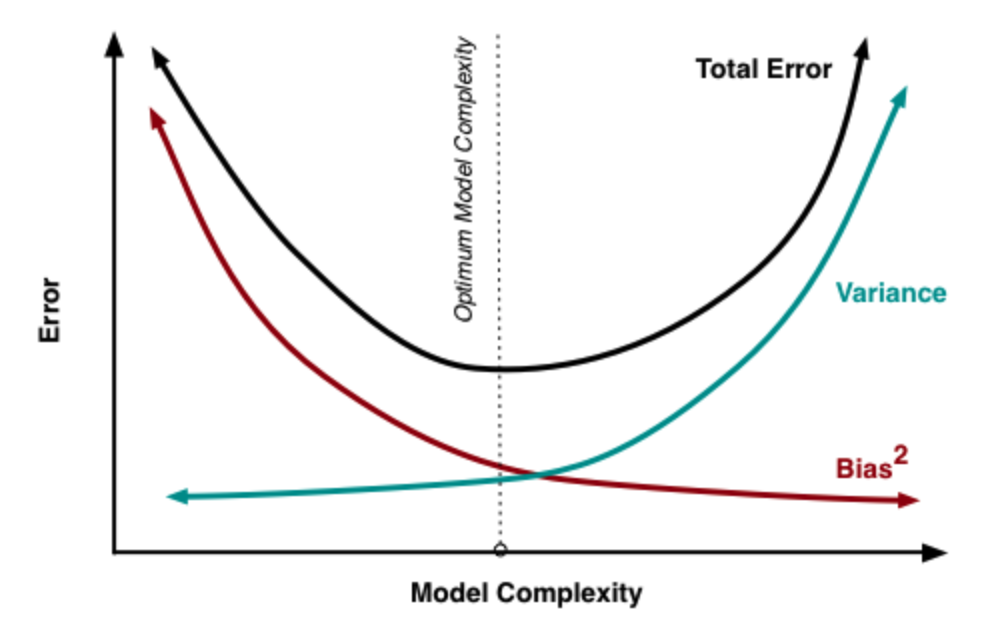
\includegraphics[width=0.5\textwidth]{../imgs/bias_variance.png}
  \end{figure}
  \item Bias($\hat{\theta}$) = $E[\hat{\theta}] - \theta$
  \item Variance($\hat{\theta}$) = $E[(E[\hat{\theta}] - \hat{\theta}])^{2}$
  \item Squared loss = $(y - \hat{y})^{2}$ where $y$ is the true value and $\hat{y}$ is the predicted value
  \item Bias-variance decomposition
  \begin{itemize}
    \item We can decompose a loss function such as the squared loss into three terms: a variance, bias, and noise term
  \end{itemize}
  \begin{align*}
    E[(y-\hat{y})^{2}] &= (y - E[\hat{y}])^{2} + E[E[(\hat{y}]-\hat{y})^{2}] \\
    &= [Bias]^{2} + Variance
  \end{align*}
  \item Decompose the 0-1 loss that we commonly use for clsasification accuracy or error
  \item \href{http://rasbt.github.io/mlxtend/user_guide/evaluate/bias_variance_decomp/}{Blog post about decomposition}
\end{itemize}

\section{Regularization}
\begin{itemize}
  \item Reduce variance to obtain more robust model
  \begin{equation*}
    \underset{\theta \in \mbb{R}^{d}}{argmin} \frac{1}{2}\sum_{i=1}^{n}(x^{(i)} \theta - y^{(i)})^{2} + \frac{\lambda}{2}\norm{\theta}^{2}_{2}
  \end{equation*}
  \begin{conditions}
    \lambda & hyperparamater \\
    \norm{\theta}^{2}_{2} & penalty for model complexity \\
    \lambda = 0 & ordinary least squares \\
  \end{conditions}
  \item Set $\lambda$ to balance bias-variance tradeoff
\end{itemize}

\section{Expectation Maximization}

\section{PCA}

\section{Support Vector Machines}
  \begin{itemize}
    \item \href{https://www.svm-tutorial.com/2014/11/svm-understanding-math-part-2/#hyperplane-equation}{svm-tutorial}
    \item Similar to logistic regression in that it is driven by a linear function $w^{T}x + b$
    \item SVMs does not provide probabilities, but outputs a class identity
    \item Given some data points, figure out the class of a new data point
    \begin{figure}[h]
        \caption{SVM}
        \centering
        \begin{subfigure}{.5\textwidth}
          \centering
          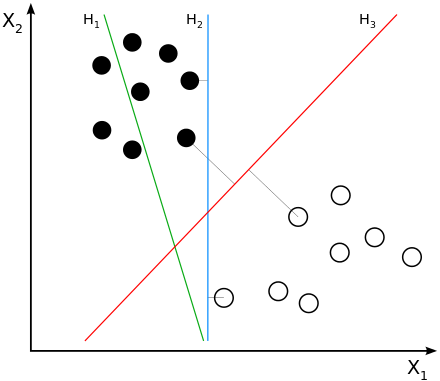
\includegraphics[width=.8\linewidth]{../imgs/svm.png}
          \label{fig:svm}
        \end{subfigure}%
        \begin{subfigure}{.5\textwidth}
          \centering
          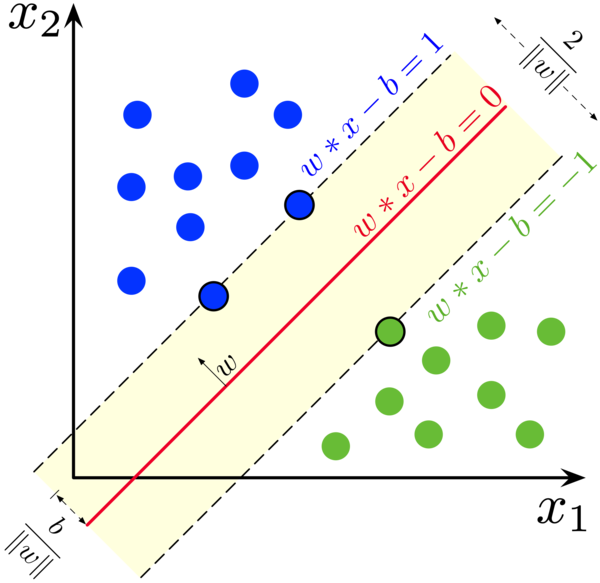
\includegraphics[width=.8\linewidth]{../imgs/svm_hyperplane.png}
          \label{fig:svm_hyperplane}
        \end{subfigure}
      \end{figure}
    \item Find the best hyperplane that represents the largest separation, or margin, between two classes
    \item Larger the margin, the lower the generalization error
    \item SVM predicts positive class then $w^{T}x+b$ is positive, else negative
    \item Kernel trick: ML algorithms can be written in terms of dot products between examples, mapping inputs to high-dimensional feature spaces
    \begin{equation*}
      w^{T}x + b = b + \sum_{i = 1}^{m} \alpha_{i}x^{T}x^{(i)}
    \end{equation*}
    \item Replace $x$ with the output of feature function $\phi(x)$ and dot product with the kernel, $k(x, x^{(i)}) = \phi(x)\cdot \phi(x^{(i)})$
    \item Apply $\phi(x)$ to all inputs and then learning a linear model in a new transformed space
    \item Gaussial kernel: $k(u,v) = \mcal{N}(u-v;0, \sigma^{2}I)$, also known as the radial basis kernel
    \item Training examples that have nonzero $\alpha_{i}$ are known as support vectors
    \item Can perform both linear and nonlinear classification using the kernel trick
    \item Hyperplane can be written in the form of a line, $y=ax+b$ or equivalently $w^{T}x - b = 0$ where $w$ is the normal vector to the hyperplane
    \item We want to find two parallel hyperplanes, "margins", that separate the two class of data so that the distance between them is as large as possible
    \item We want
    \begin{align*}
      w^{T}x - b &= 1 \\
      w^{T}x - b &= -1 \\
    \end{align*}
    \item Training objective: minimize $\norm{w}$ subject to $y_{i}(w^{T}x_{i} - b) \geq 1 for i = 1, \dotsc, n$
    \item These constraints say that data points much lie on the correct side of the margin
  \end{itemize}

\section{Precision v.s. Recall}
  \begin{itemize}
    \item Precision (positive predictive value): the fraction of relevant instances among retrieved instances
    \item Recall (sensitivity): fraction of total amount of relevant instances that were retrieved
    \item F-measure: harmonic mean of precision and recall
    \begin{align*}
      \text{precision} &= \frac{tp}{tp+fp} \\
      \text{recall} &= \frac{tp}{tp+fn} \\
      \text{f-score} &= 2 \cdot \frac{\text{precision} \cdot \text{recall}}{\text{precision} + \text{recall}}
    \end{align*}
    \begin{figure}[h]
      \caption{Confusion Matrix}
      \centering
      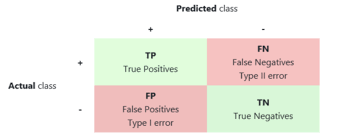
\includegraphics[width=0.8\textwidth]{../imgs/confusion_matrix.png}
    \end{figure}
    \item Type I error: false positive, Type II error: false negative
    \item Precision-recall tradeoff
    \item Precision is more important than recall when you would like to have less false positives in tradeoff to have more false negatives. Getting a false positive is very costly, and a false negative not as much
    \item For example, in a zombie apocalypse, you want to accept as many healthy people in the safe zone. Don't want to mistaken pass a zombie into safe zone (aka false positive). It's fine if some of the healthy people don't get into safe zone (aka false negative)
    \item Recall is more important when you want to capture all the positive cases. It is most costly to miss a positive than including a negative. Very important for medical purposes
    \item For example, we're more willing to tell someone they have a cancer than to let a positive slip through the crack. We don't care about false positives, but we want to get all the positives possible
    \item Accuracy is not a good metric when there is heavy class imbalance
    \item ROC plots the true positive rate against the false positive rate at various thresholds
    \item Area under ROC (AUROC)
  \end{itemize}


\section{Information Theory}
\subsection{Entropy}
  \begin{itemize}
    \item Entropy of a random variable is the average level of "information", "surprise", or "uncertainty" in the variables possible outcomes.
    \begin{equation*}
      H(X) = -\sum_{i=1}^{n} P(x_{i})\text{log}{P(x_{i})}
    \end{equation*}
    \item Created by Shannon as part of theory of communication
    \item Entropy is 0 means that the outcome is always certain, no new information
  \end{itemize}
\label{sub:entropy}

\subsection{Cross Entropy} % (fold)
\label{sub:cross_entropy}

% subsection cross_entropy (end)

\subsection{KL Divergence} % (fold)
\label{sub:kl_divergence}
  \begin{itemize}
    \item Measure of how one probability distribution is different from a second
    \item For two probability distributions $P$ and $Q$
    \begin{equation*}
      D_{KL}(P||Q) = \sum_{x \in \mcal{X}} P(X) log(\frac{P(x)}{Q(x)}) = \sum_{x \in \mcal{X}} P(X) log(\frac{Q(x)}{P(x)})
    \end{equation*}
    \item $D_{KL}(P||Q)$ is often called the \textit{information gain} if $P$ were used instead of $Q$, it is also called the \textit{relative entropy} of $P$ wrt $Q$
    \item KL divergence is always non-negative, also known as Gibb's inequality, $D_{KL}(P||Q) \geq 0$
    \item KL divergence is not symmetric, hence it cannot be a "distance metric", $D_{KL}(P||Q) \neq D_{KL}(Q||P)$
  \end{itemize}

% subsection kl_divergence (end)

\subsection{Mutual Information} % (fold)
\label{sub:mutual_information}
  \begin{itemize}
    \item hehehehe
    \begin{equation*}
      I(X;Y) = D_{KL}(P(X, Y) || P(X)P(Y))
    \end{equation*}
  \end{itemize}
% subsection mutual_information (end)

\section{Decision Trees} % (fold)
\label{sec:decision_trees}

% section decision_trees (end)

\section{K Nearest Neighbors} % (fold)
\begin{itemize}
  \item non-parametric method used for classification and regression
  \item in classification the output is class membership: an object is classified by plurality vote of neighbors (mode)
  \item in regression, the output is a property value of an object, usually the average of its k-nearest neighbors
  \item compute distance between a query point and all other examples in the data, and selecting the K closest and take a vote or average depending on the problem
  \item distance metrics:
  \begin{itemize}
    \item Euclidean distance
    \item Taxicab / manhattan distance
    \item Minkowski distance
    \item Jaccard index
    \item Hamming distance
  \end{itemize}
  \item no need to build model, tune parameters
  \item KNN doesn't scale well as the number of examples increases
\end{itemize}
\label{sec:knn}
% section knn (end)

\section{Logistic Regression}
  \begin{itemize}
    \item a statistical model that uses a logistic function to model a binary dependent variable
    \item linear regression doesn't work for classification because a linear model doesn't output probabilities, also doesn't scale to classification problems with multiple classes
    \item logistic function
    \begin{equation*}
      \text{logistic}{(n)} = \frac{1}{1 + \text{exp}(-n)}
    \end{equation*}
    \item the logistic function forces the output to assume values between 0 and 1
    \item
    \item Multinomial (softmax) Logistic Regression
  \end{itemize}

\section{Gradient Descent}

\section{Optimizers}

\section{Weak supervision}

\section{Transfer Learning}
\begin{itemize}
  \item
\end{itemize}

\section{Graph of various useful functions}
\begin{figure}[h]
  \caption{Important functions}
  \centering
  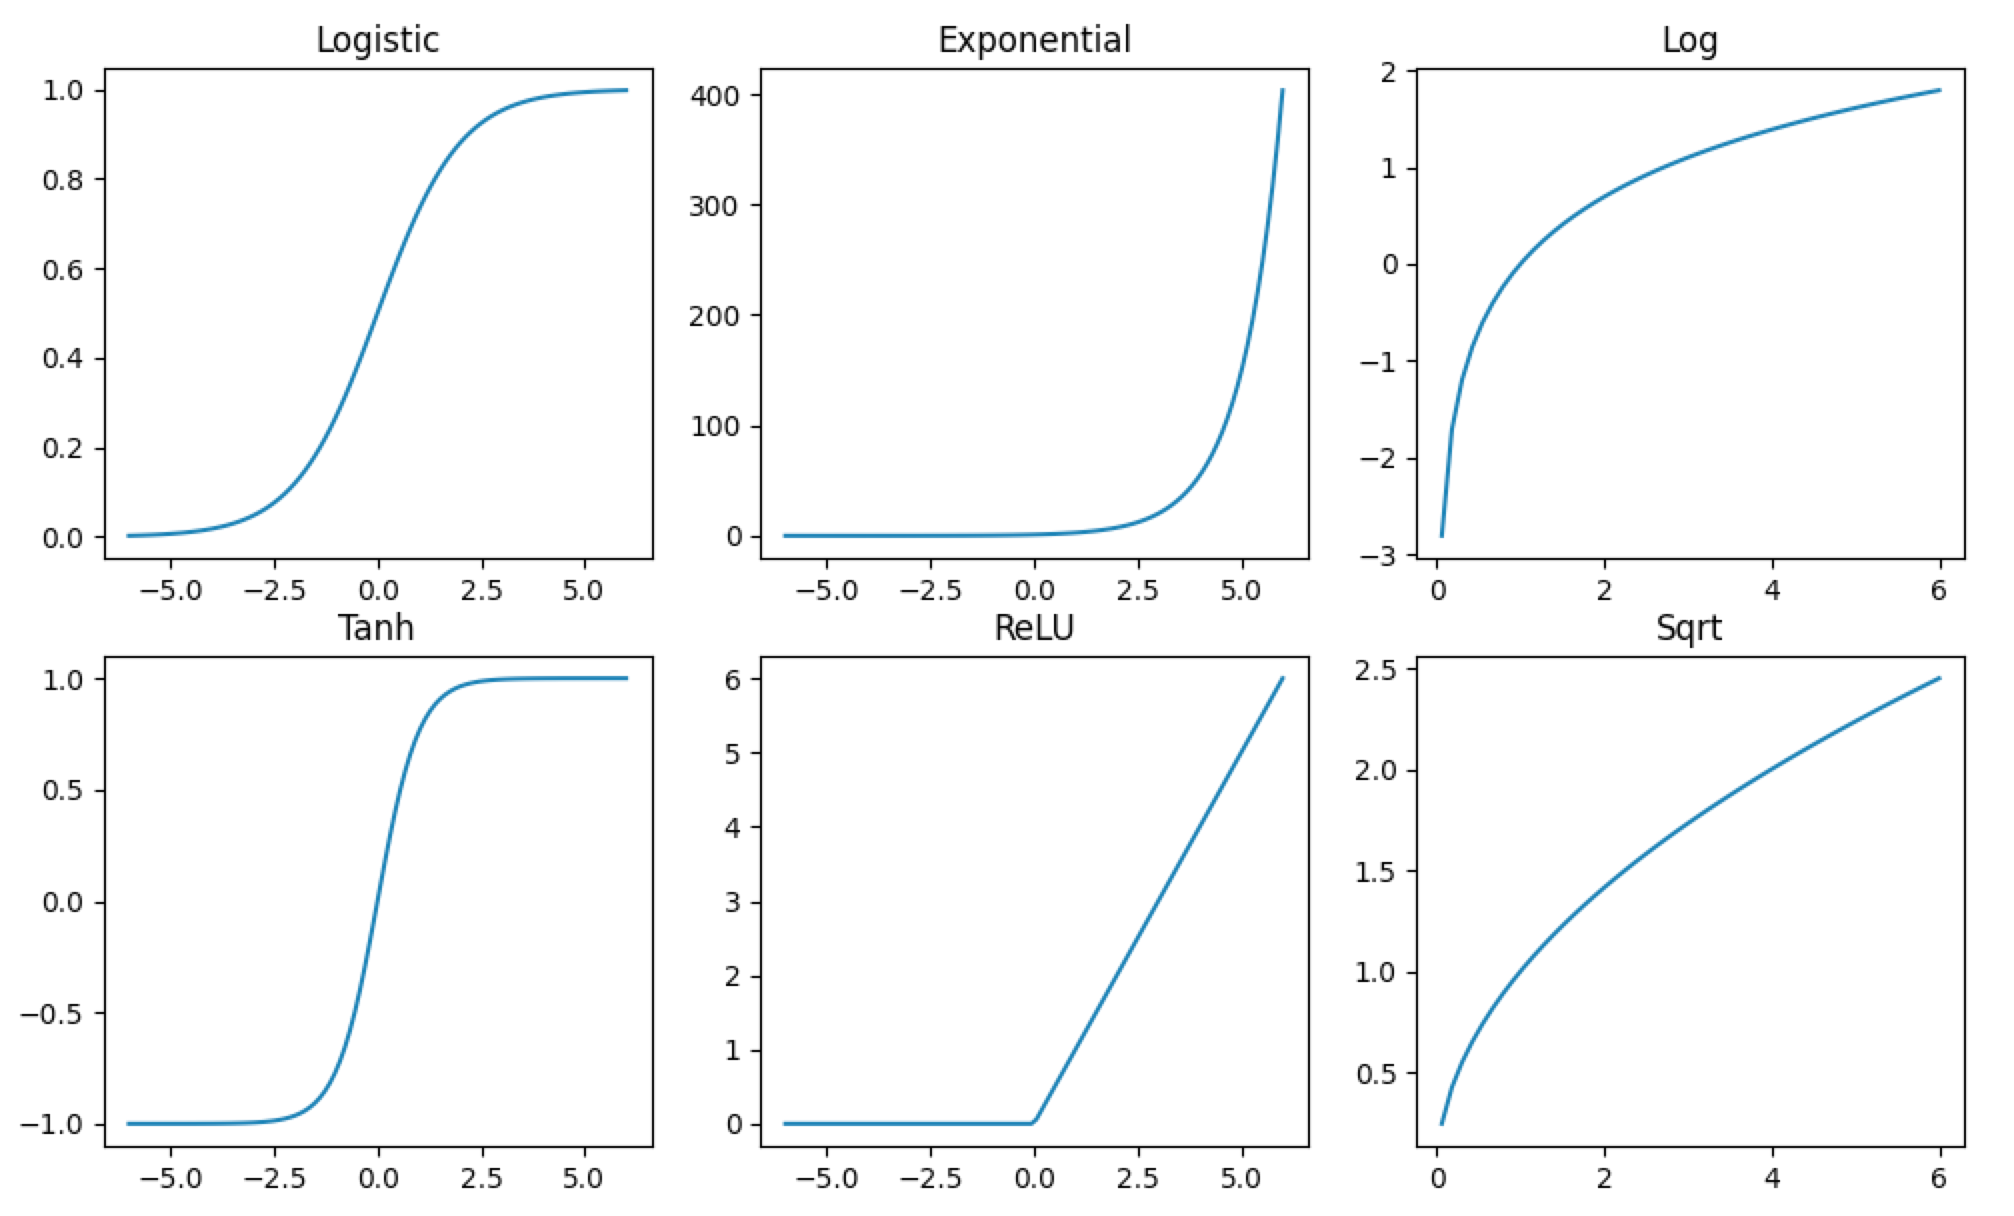
\includegraphics[width=1\textwidth]{../imgs/functions.png}
\end{figure}

\section{ML Tips and Advice}

7 Steps to ML
\begin{enumerate}
  \item Acquire data
  \begin{itemize}
    \item hidden data artifacts are challenging
  \end{itemize}
  \item Look at your data!
  \begin{itemize}
    \item always look at your data!
    \item have the right people look at your data (e.g. physicians)
  \end{itemize}
  \item Create train/dev/test splits
  \begin{itemize}
    \item Fit model to training dataset
    \item Fit hyperparameters to validation or development dataset
    \item Test model performance on test set
    \item Avoid leakage and adaptive overfitting
    \item Splits should be randomly sampled, but depends on application
  \end{itemize}
  \item Create a specification
  \begin{itemize}
    \item A good specification has little ambiguity
  \end{itemize}
  \item Build a model (simplest that works!)
  \begin{itemize}
    \item Try linear of logistic regression w/ simple features
    \item Good baseline for future work
    \item Avoid getting bogged down in new models, use them to understand the data
    \item Ablation studies: figure out which part matters and which parts are stable
    \item Remove one feature at a time
    \item What could be wrong?
    \begin{itemize}
      \item Maybe it's the data or your features? Try get more training data. Try smaller set of features. Try adding more features.
      \item Maybe it's the optimization algorithm? Try running GD longer. Try SGD, GD, Newton, etc.
      \item Maybe it's the hyperparamters?
      \item Try different model?
    \end{itemize}
  \end{itemize}
  \item Measurement
  \begin{itemize}
    \item Measure end-to-end quality metrics
    \item Automatic monitoring
    \item Labels and input drift (change) over time
    \item Variance diagnostics - use k-fold cross validation and check that dev scores have small relative error
  \end{itemize}
  \item Repeat

  \item Lasso path: sweep regularize parameter for L1, train the model, and see when features turn on
  \item
  \begin{figure}[h]
    \caption{Techniques for limited labeled data}
    \centering
    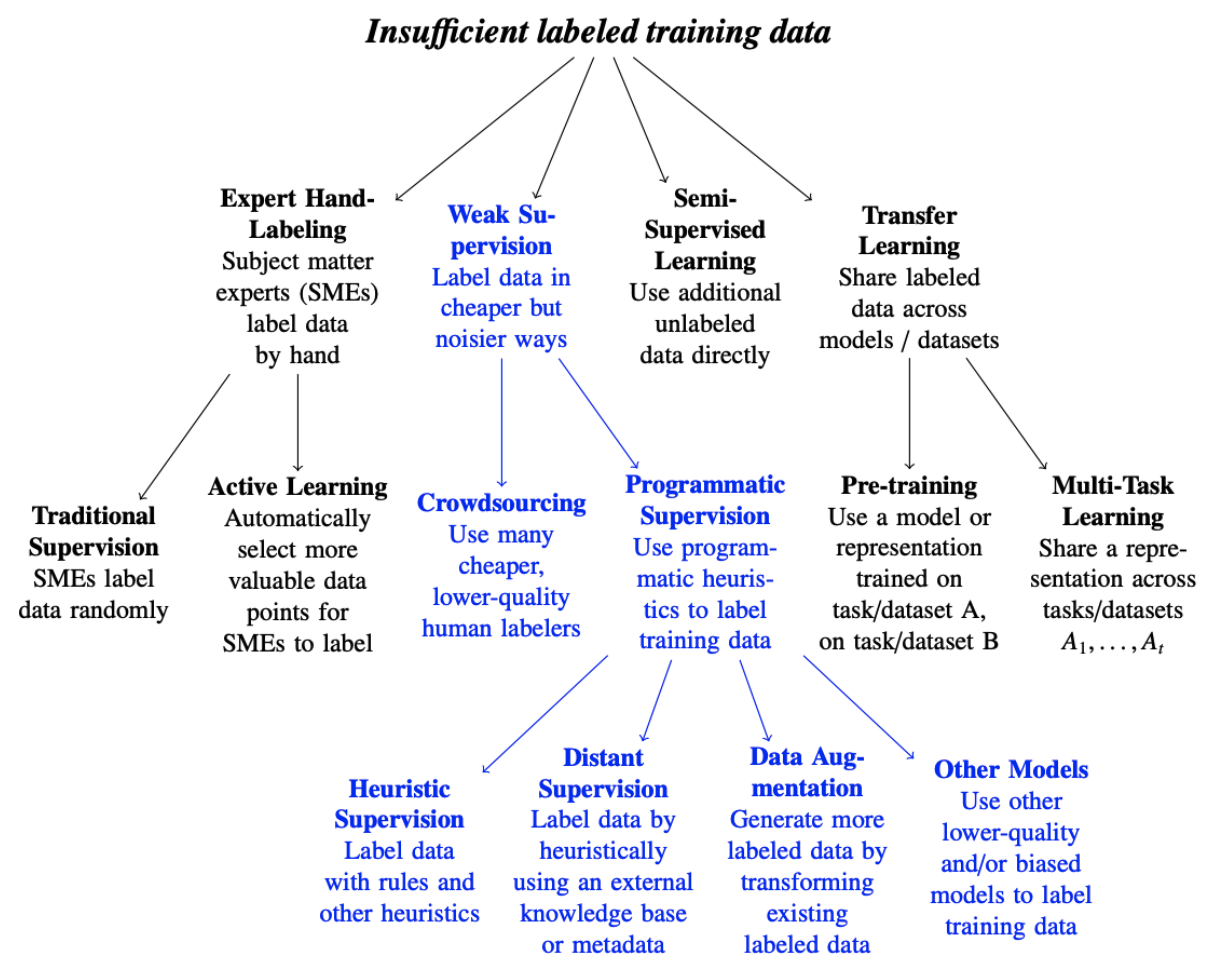
\includegraphics[width=0.5\textwidth]{../imgs/ml.png}
  \end{figure}
\end{enumerate}



\end{document}